\documentclass[a4paper,12pt,draft]{article}

\usepackage{enumitem}
\usepackage[utf8]{inputenc}
\usepackage{textcomp}
\usepackage{xspace}
\usepackage[italian]{babel}
\usepackage[pdftex,final]{graphicx}
\usepackage{fullpage}
\usepackage{amsmath}
\usepackage{subfig}
\usepackage{multirow}
\usepackage{booktabs} % alcune caratteristiche aggiuntive tabelle

\usepackage{listings}
\lstset{
	basicstyle=\fontsize{8}{12}\ttfamily,
	inputencoding=utf8,
	language=Java,
	numbers=left,
	numberstyle=\tiny,
	tabsize=2,
	frame=single,
	backgroundcolor=\color{gray},
}

\setenumerate[2]{label=\alph*.}

\usepackage{color}
\definecolor{gray}{gray}{0.9}

\usepackage[final]{hyperref}
\hypersetup{
	colorlinks=true
}
\usepackage{hypcap}

\newcommand{\ddbp}{$2D -$\emph{bin packing}}
\newcommand{\ddbpp}{problema \ddbp{}}

\begin{document}

\thispagestyle{empty}
\begin{center}
	\leavevmode
	\large
	\begin{tabular}{ r l }
		\multirow{2}{*}{\includegraphics[width=2cm]{img/unipd_logo.png}} & \textsc{Università degli studi di Padova}\par \\
			& \textsc{Corso di laurea magistrale in Ingegneria Informatica} \\
	\end{tabular}
	\vskip 3cm
	
	\vfill
	\textbf{{\large Relazione del progetto del corso di Intelligenza Artificiale}}\\[0.2cm]
	\textbf{{\LARGE Approcci metaeuristici al 2D Bin Packing Problem}}\par
	\vskip 3cm
	\normalfont
	
	\begin{tabular}{ c c c }
		\large Luca \textsc{Gasparini} & Alberto \textsc{Boccato} &
				Nicola \textsc{Chessa} \\
		\normalsize 999999 & 999999 & 999999 \\
	\end{tabular}
	\vskip 0.5cm
	\begin{tabular}{ c c }
		\large Nicola \textsc{Dalla Benetta} & Nicola \textsc{Gobbo} \\
		\normalsize 999999 & 1014195 \\
	\end{tabular}
	\normalfont
	\vskip 4cm
	
	\begin{flushright}
		\emph{Docente:}\\
		Prof. Silvana \textsc{Badaloni}\\
	 \vskip 2cm
		\emph{Collaboratori:}\\
		Dott. Francesco \textsc{Sambo}\\
	\end{flushright}

	
	\vfill
	{\large A.A. 2011-2012}
\end{center}
\cleardoublepage

\begingroup
	\hypersetup{linkcolor=black}
	\setcounter{tocdepth}{2}
	\tableofcontents
\endgroup

\newpage

\section{Introduzione}
Lo scopo di tale relazione è quello di illustrare alcuni algoritmi
metaeuristici per risolvere il problema del \ddbp{}; in particolare
attraverso l'euristica Bottom-Left-Fill (BLF) si sono scelti i seguenti:
\begin{itemize}
\item Genetico;
\item Genetico basato su torneo
\item Tabu Search.
\end{itemize}
Inoltre si è realizzata l'interfaccia grafica per ottere un supporto che
evidenziasse il comportamento di tali algoritmi.

\subsection{Descrizione del problema}
Il \ddbpp{} (2-DBPP) con rotazioni è definito come segue:
\begin{itemize}
\item dato un insieme di n oggetti rettangolari di dimensioni $h_{i}$ e $w_{i}$
che rappresentano rispettivamente l'altezza e la larghezza dell’oggetto
i-esimo;
\item dato un insieme illimitato di contenitori, ognuno dei quali ha altezza
H e larghezza W;
\end{itemize}
Minimizzare il numero dei contenitori (nBin) utilizzati a seguito
dell'inserimento di tutti gli oggetti senza sovrapposizione (nBIN) è
l'obbiettivo del problema. Gli oggetti possono essere ruotati di 90 gradi,
questo aumenta le dimensioni dello spazio di ricerca e quindi la difficolta’ per
raggiungere la soluzione ottima, ma produce il vantaggio di ridurre il numero di
contenitori necessari.
I vincoli cui devono sottostare gli algoritmi risolutivi sono i seguenti:
\begin{itemize}
 \item ogni oggetto deve essere inserito in un solo bin;
 \item le dimensioni di ogni singolo oggetto devono essere minori delle
dimensioni del bin;
 \item le dimensioni dell'area totale occupata dalla somma degli oggetti in un
bin deve essere inferiore all'area del bin.
\end{itemize}
Tali vincoli sono necessari altrimenti la soluzione del problema è triviale,
infatti il problema non avrebbe alcuna soluzione.

\subsection{Descrizione generale di un algoritmo per 2-DBPP}
Ogni algoritmo utilizzato in questa relazione ha la seguente struttura.

INPUT:
\begin{itemize}
  \item H e W dimensioni di tutti i bin;
  \item $h_{i}$ e $w_{i}$ dimensioni dell’oggetto i-esimo;
\end{itemize}

OUTPUT:
\begin{itemize}
 \item nBIN numero di bin necessari per contenere gli oggetti;
 \item posizionamento degli oggetti in ogni bin con rappresentazione grafica;
 \item numero delle soluzioni ottime;
 \item tempo di esecuzione;
\end{itemize}

Il 2-DBPP è un problema NP-Completo, ovvero fa parte di quella classe di
problemi per i quali non è possibile, in tempo polimoniale, ottenere una o più
soluzioni ottime.
Proprio da questo aspetto nasce l'esigenza di ottenere buone soluzioni
approssimate che siano ragionevolmente vicine all'ottimo; tali soluzioni si
possono ottenere attraverso la coniugazione di euristiche particolari e
algoritmi metaeuristici. 

\section{Euristica Bottom-Left-Fill}
Una delle euristiche più utilizzate per risolvere il \ddbpp{} è la \emph{bottom-left} (BL), che consiste nel prendere uno ad uno in un certo ordine i pacchetti da inserire nel bin e farli cadere il più in basso possibile per poi spostarli più a sinistra possibile, trovando una posizione valida quando il pacchetto appoggia su una superficie sia a sinistra che in basso. Questa euristica è particolarmente importante in quanto è stato dimostrato \cite{BLTheorem} che se esiste un modo per disporre un certo insieme di pacchetti in un \emph{bin} esiste anche una permutazione dell'insieme che permette di inserire tali pacchetti nel suddetto bin tramite l'euristica BL. Prendendo quindi un \emph{bin} delle dimensioni minime per contenere la soluzione ottima è possibile dimostrare che questa è ottenibile tramite l'algoritmo BL.

L'algoritmo BL in media però non è molto efficiente in quanto può lasciare degli spazi vuoti che se vengono chiusi da un pacchetto non possono più essere utilizzati nei passi successivi dell'algoritmo. Per risolvere questo problema è stata ideata la variante Bottom-Left-Fill (BLF) che consiste nell'inserire ogni pacchetto nella posizione più in basso possibile considerando anche le posizioni all'interno dei buchi lasciati dal placing dei pacchetti precedenti. A parità di altezza vengono privilegiate le posizioni più a sinistra. Il BLF si presta bene all'utilizzo combinato con algoritmi genetici in quanto associa una permutazione dei pacchetti ad un particolare placing degli stessi e garantisce che almeno una delle permutazione conduca ad un placing ottimo. Si può perciò pensare di utilizzare come cromosoma una sequenza ordinata di pacchetti (eventualmente ruotati) ed applicare ad essa mutazioni e cross-over order-based per giungere ad una soluzione di fitness massima.

Pur essendo un'euristica molto semplice a livello intuitivo, l'implementazione naive di questo algoritmo richiede tempo $O(n^4)$ nel numero di pacchetti, in questo progetto invece abbiamo deciso di utilizzare l'implementazione proposta da Chazelle \cite{chazelleBL} che richiede spazio lineare e tempo $O(n^2)$ nel numero di pacchetti. In questa sezione verrà descritta l'idea alla base dell'algoritmo ideato da Chazelle e le nostre scelte implementative. 

\subsection{Descrizione dell'algoritmo}
Ad ogni stadio dell'algoritmo BLF, ogni \emph{bin} contiene degli spazi vuoti detti \emph{hole}, che possono essere visti come poligoni formati da solo lati orizzontali e verticali. L'algoritmo procede esaminando uno alla volta gli \emph{hole} e determinando tutte le posizioni in cui può essere inserito il rettangolo corrente, per poi scegliere la posizione più in basso a sinistra. Ogni hole viene rappresentato con una lista dei suoi lati. Un lato di un hole viene detto \emph{leftmost edge} se forma, con i due lati ad esso adiacenti, due angoli convessi ed entrambi i due lati giacciono alla sua destra. Al contrario, un lato di un hole viene detto un \emph{notch} se forma, con i due lati ad esso adiacenti, due angoli concavi. Un \emph{notch} verticale in particolare viene detto \emph{left notch} se i due lati ad esso adiacenti giacciono alla sua sinistra. Infine, un angolo concavo con al di sopra un lato verticale e un lato orizzontale alla sua destra viene detto \emph{falling corner}.
Per prima cosa, per ogni hole bisogna individuare tutti i \emph{left notch} e i \emph{leftmost edge} ad essi associati e suddividere l'\emph{hole} nei relativi \emph{sub-hole} nel modo rappresentato in figura \ref{fig:imgBLF1}.

\begin{figure}[h!tp]
 \centering
 \includegraphics[width=0.8\textwidth]{./img/imgBLF1.pdf}
 % imgBLF1.pdf: 584x347 pixel, 72dpi, 20.60x12.24 cm, bb=0 0 584 347
 \caption{Individuazione dei \emph{left notches} e \emph{leftmost edge} associati.}
 \label{fig:imgBLF1}
\end{figure}

Si può dimostrare che ognuno di questi \emph{sub-hole} è \emph{nice} cioè non contiene left, right o upper \emph{notch} e contiene al massimo un \emph{falling corner}. Una volta ottenuti dei \emph{sub-hole} di questo tipo, possiamo, in tempo lineare, trovare tutte le posizioni dove può essere inserito il pacchetto all'interno del \emph{sub-hole}.
Definiamo $FB$ la lista dei punti che delimitano la parte inferiore del \emph{sub-hole} ed $FT$ quella dei punti che ne delimitano la parte superiore. 
Per prima cosa pensiamo di rimuovere la \emph{linea poligonale} corrispondente ad $FT$, ottenendo quindi un area $A$ infinita delimitata inferiormente da $FB$. Consideriamo ora un segmento $(b1,b2)$ di lunghezza pari a quella del rettangolo da inserire. Dobbiamo trovare tramite la procedura \texttt{Bottom}, l'insieme dei punti $C$ tali che, $p \in C$ se, considerando la verticale dove giace $p$, esso è il punto $b1$ con coordinata $y$ minima tale che il segmento $(b1,b2)$ giace interamente nell'area $A$.
Consideriamo ora l'area $B$ infinita, delimitata superiormente da $FT$ e troviamo l'insieme dei punti $D$ di coordinata $y$ massima tali che il segmento sia contenuto interamente in $B$. Questi due insiemi possono essere trovati in tempo lineare scorrendo le relative liste $FB$ e $FT$.

\begin{figure}[h!tp]
 \centering
 \includegraphics[width=0.8\textwidth]{./img/imgBLF2.pdf}
 % imgBLF2.pdf: 962x432 pixel, 72dpi, 33.94x15.24 cm, bb=0 0 962 432
 \caption{}
 \label{fig:imgBLF2}
\end{figure}

A questo punto, per trovare i punti dove è possibile inserire il rettangolo basta scorrere da sinistra a destra contemporaneamente i due insiemi e riportare come feasible i punti di $C$ tali che la differenza di altezza con il punto di $D$ nella stessa verticale sia maggiore dell'altezza del rettangolo. Il tutto può essere eseguito ancora una volta in tempo lineare nel numero di pacchetti già inseriti. L'algoritmo che inserisce uno alla volta tutti i pacchetti risulterà quindi essere di complessità $O(n^2)$.

\section{Tabu Search}
Il \textit{Tabu search} é un algoritmo meta euristico di ricerca locale. La differenza principale rispetto all'algoritmo genetico é che, durante la sua esecuzione, tiene traccia delle soluzioni calcolate e non solo dell'ultima trovata. Da questo si può intuire come la memoria e la sua gestione giochi un ruolo chiave in questo tipo di approccio. Ad ogni iterazione, l'algoritmo cerca di trovare la soluzione più conveniente, anche se questa é una mossa peggiorativa rispetto all'ultima soluzione trovata. Il motivo per la quale si accettano soluzioni peggiori è per evitare che l'algorimo si soffermi in un ottimo locale; tuttavia, così facendo, c'è il pericolo che l'algoritmo vada in stallo a causa di cicli: per questo motivo viene introdotta una lista tabu all'interno della quale vengono memorizzate le mosse proibite, ovvero le ultime mosse calcolate. Indicando con $l_t$ la lunghezza della lista tabù, così facendo si evitano cicli di dimensioni $\le l_t$. Quindi nel \textit{tabu search}, l'ultima soluzione trovata dipende dalle soluzioni precedenti e dall'intorno della soluzione stessa.
   
Di seguito verrà esposto come é stata implementata questa strategia per risolvere il problema del \ddbp.

\subsection{Algoritmo}
In questa sezione verrà esposto lo pseudocodice utilizzato e verranno spiegate le funzionalità.
L'algoritmo inizia la sua esecuzione partendo da una soluzione ammissibile del problema: la soluzione ammissibile scelta corrisponde a inserire ciascun pacchetto in un bin diverso, di conseguenza inizialmente il numero di contenitori totale equivale al numero di pacchetti. Successivamente, ad ogni iterazione l'algoritmo cerca di migliorare la soluzione corrente effettuando una mossa migliorativa cercando tra le soluzioni vicine.

La mossa migliorativa viene scelta secondo il seguente criterio: l'algoritmo deve determinare il bin che é più facilmente svuotabile (\textit{bin target}) e, preso un pacchetto $j$ appartenente al \textit{bin target}, si cerca di modificare un insieme S di pacchetti in modo tale da aggiungere il pacchetto $j$ a $S$. Il sottoinsieme $S$ viene creato prendendo i pacchetti presenti nei $k$ bin iniziali ecluso il \textit{bin target}. L'intero $k$ determina la dimensione dei vicini; per esempio, con $k=1$, l'insieme $S$ é formato dal contenuto di un altro bin e il pacchetto $j$, con $k=2$, l'insieme $S$ é formato dai pacchetti presenti in due bin più e il pacchetto $j$, e così via.

La dimensione del valore $k$ é importante per due motivi:
\begin{enumerate}[noitemsep]
\item indica la dimensione delle soluzioni vicini da navigare;
\item influisce sulla velocità di esecuzione dell'algoritmo: con $k=t$, al caso pessimo si dovranno creare al più $2^{t}$ insiemi;
\end{enumerate}



L'algoritmo di placing utilizzato per posizionare i pacchetti all'interno del bin é BLF (Bottom Left Fill); 

\texttt{\footnotesize
   \begin{tabbing}
   \=~~~\=~~~\=~~~\\
   \>\%pseudocodice
   \end{tabbing}
}


% \cite{lmvTabu}
% \cite{lmvTspack}
\section{Framework di esecuzione}
Il programma sviluppato è stato progettato con l'obiettivo di fornire un framework di esecuzione per algoritmi che risolvono il \ddbpp. L'intento è creare un ambiente in cui, lo sviluppatore che voglia verificare le performance di un nuovo algoritmo, possa concentrarsi solo sullo sviluppo dello stesso, senza preoccuparsi di tutte le problematiche relative alla grafica o alla \emph{user experience}.

\subsection{Aspetto}
Ad un utente finale l'interfaccia grafica si presenta come in figura \ref{fig:main_window_ss}. Da questa finestra è possibile configurare le specifiche del problema quale dimensione dei contenitori, o \emph{bin}, e il numero di pacchetti, o \emph{packet}, con relative larghezze e altezze. Una volta configurato il problema, si potrà scegliere l'algoritmo, o \emph{Core}, con il quale risolverlo: ogni metodo risolutivo ha parametri di configurazione propri, mostrati nella sezione loro dedicata, che possono venir usati per adattare il comportamento dell'algoritmo alla specifica istanza. Una volta completata la fase di configurazione il \emph{Core} può essere lanciato e, ad ogni ottimo trovato, ne verrà visualizzato il \emph{placing}, il valore di fitness, il numero di iterazioni e il tempo impiegato per raggiungerlo.

\begin{figure}[h!tp]
 \centering
 \includegraphics[width=\textwidth]{./img/main_window_ss.png}
 % main_window_ss.png: 1160x709 pixel, 72dpi, 40.92x25.01 cm, bb=0 0 1160 709
 \caption{Screenshot della finestra principale del programma}
 \label{fig:main_window_ss}
\end{figure}

\subsection{Caratteristiche peculiari}
Il framework sviluppato mette a disposizione diverse caratteristiche per facilitare l'utente finale nell'uso del software, così come lo sviluppatore nel test degli algoritmi.
\paragraph{Salvataggio \& caricamento della configurazione corrente}
Attraverso i pulsanti \texttt{SAVE} e \texttt{LOAD CONFIGURATION} è possibile salvare o caricare da file la configurazione del problema attualmente in esame, comprensiva del core selezionato e dei suoi parametri specifici. Il file prodotto sarà formattato secondo lo standard XML e modificabile anche al di fuori del programma.
\paragraph{Cronologia degli ottimi}
Ogni volta che l'algoritmo individua un nuovo ottimo la sua rappresentazione prende il posto della precedente. Questo comportamento può non essere sempre gradito in quanto uno sviluppatore potrebbe voler vedere l'intera evoluzione degli ottimi, per capire se l'algoritmo scritto si comporta nel modo correto, mentre un utente potrebbe accorgersi che, per una non precisa calibrazione della funzione di fitness, un ottimo precedente risulta ``più adatto agli scopi'' di quello successivo. Per porre rimedio a questo ostacolo il framework salva l'intera cronologia degli ottimi che possono così essere visualizzati nuovamente.
\paragraph{Salvataggio \& caricamento di ottimi}
I pulsanti \texttt{EXPORT} e \texttt{LOAD OPTIMUM} permettono all'utente di salvare qualsiasi ottimo presente nella cronologia, nonchè visualizzarlo nuovamente in futuro. Il file prodotto contiene la sequenza di bin con il \emph{placing} dei relativi pacchetti e, essendo in formato XML, può essere facilmente interpretato da un programma di terze parti.
\paragraph{Ingrandimento automatico dei \emph{bin}}
Da un punto di vista esclusivamente di \emph{user experience} la rappresentazione grafica dei \emph{bin} viene riscalata ogni volta che le dimensioni della finestra, e dei \emph{bin} stessi, lo permettono. Ciò facilita l'analisi dell'ottimo trovato soprattutto quando questo è composto da oggetti di piccole dimensioni.

\subsection{Classi essenziali}
L'aggiunta di nuovi \emph{Core} da parte di uno sviluppatore comincia con la comprensione dello schema UML presentato in figura \ref{fig:uml_classi}.
\begin{description}
	\item[\texttt{MainWindow}]
	\item[\texttt{ProblemConfiguration}] La creazione e gestione di questa classe è demandata 
	\item[\texttt{GUISignaler}]
	\item[\texttt{OptimumPainter}]
	\item[\texttt{CoreDescriptor}]
	\item[\texttt{CoreController}]
	\item[\texttt{AbstractCore \& SwingWorker}]
	\item[\texttt{AbstractConfigurator}]
\end{description}


\begin{figure}[h!tp]
 \centering
 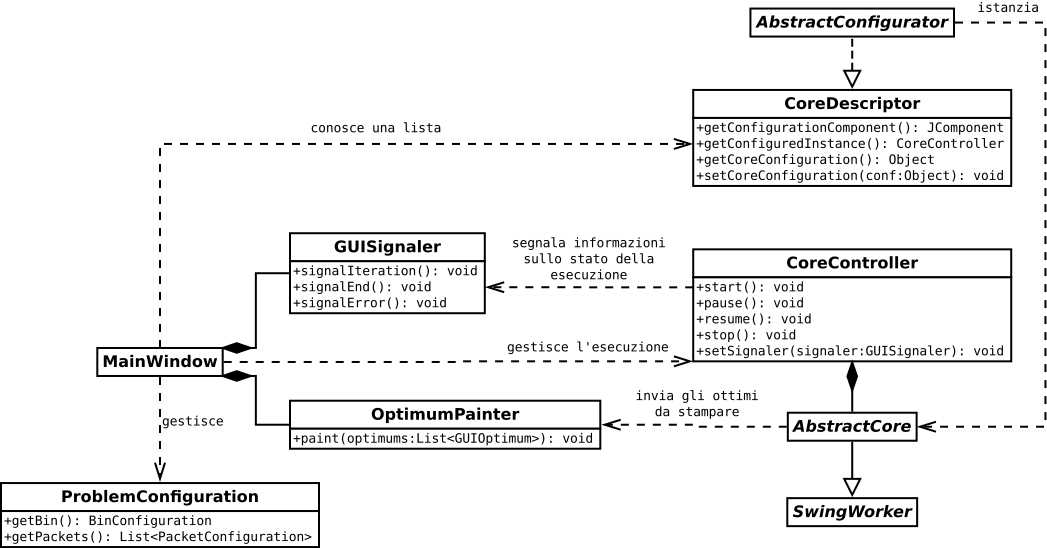
\includegraphics[width=\textwidth]{./img/uml_classi.pdf}
 % uml_classi.pdf: 1047x548 pixel, 72dpi, 36.94x19.33 cm, bb=0 0 1047 548
 \caption{Grafico UML delle classi principali dell'applicazione}
 \label{fig:uml_classi}
\end{figure}


\section{Conclusione}
Dall'esperienza accumulata sviluppando questo progetto è stato valutato che gli algoritmi metaeuristici, nella fattispecie \emph{genetico} e \emph{tabu search}, si comportano bene nella soluzione del \ddbpp. Osservando gli ottimi proposti si nota che in poco tempo ci sono ``andati molto vicini'' seppure si notano comunque possibili margini di miglioramento. Pensando in un ottica di applicazione commerciale questo comportamento è favorevole in quanto risulta più facile ottimizzare un problema partendo già da una soluzione sub-ottima che in poco tempo è riuscita ad individuare pattern particolari.

Confrontando i due \emph{Core} a nostra disposizione la prima differenza che salta all'occhio è nel numero di paramentri: l'algoritmo \emph{genetico} richiede una configurazione più ampia che cambia da un'istanza all'altra, mentre il \emph{tabu search} offre parametri con validità più generale. Detto ciò il \emph{tabu search} risulta essere più intuitivo per la logica umana mentre il \emph{genetico} sembra più casuale nella sua evoluzione ma, dai test effettuati, risulta comportarsi meglio su istanze che coinvolgono pochi bin mentre i due algoritmi tendono a produrre soluzioni equivalenti con l'aumentare del numero di bin necessari.

In rete è possibile trovare programmi commerciali\footnote{In particolare abbiamo individuato il programma \emph{2D Load Packer} della Astrokettle Algorithms (\url{http://www.astrokettle.com/pr2dlp.html}) che forniva una libreria di istanze risolte, usate come metrica di riferimento.} che risolvono il problema del \ddbp, si è deciso quindi di confrontarsi con tali programmi su medesime istanze per valutare la bontà del codice prodotto, è emerso che per quasi tutte le istanze i risultati da noi ottenuti sono molti vicini a quelli ottenibili con i software commerciali. Questo evidenzia il fatto che con particolari accorgimenti potrebbe esser possibile migliorare leggermente quanto ottenuto, le tipologie di algoritmi per problemi quali il \ddbp sono infatti molto sensibili a particolari accorgimenti come ordinamenti o euristiche distinte adottate.

Il programma sviluppato è distribuito sotto licenza GNU GPLv3\footnote{\url{http://www.gnu.org/licenses/gpl.html}} e liberamente scaricabile dal sito \url{https://code.google.com/p/iaproject-2dbpp/}.


\phantomsection
\addcontentsline{toc}{section}{Bibliografia}
\bibliographystyle{plain}
\bibliography{IABibliography}

\end{document}
